% !TeX spellcheck = cs_CZ
\documentclass[a4paper,11pt,titlepage,fleqn]{article}

\usepackage[utf8]{inputenc}
\usepackage[top=2.5cm, bottom=2.5cm, left=3.5cm, right=2.5cm]{geometry}
\usepackage[czech]{babel}
\usepackage[IL2]{fontenc}  
\usepackage{graphicx}
\usepackage[nonumberlist,acronym]{glossaries}
\usepackage{cite}
\usepackage{fancyhdr}
\usepackage{afterpage}
\usepackage[hidelinks,unicode,hyperfootnotes]{hyperref}
\usepackage{footnote}
\usepackage{parskip}
\usepackage{setspace} 
\usepackage{listings}
\usepackage{pdfpages}
\usepackage{dirtree}
\usepackage{booktabs}
\usepackage{amsmath}
\usepackage{nccmath}
%\usepackage[T1]{fontenc}
%\usepackage[bottom]{footmisc}
%\usepackage{fancyvrb}

\lstset{
    language=PHP,
    basicstyle=\ttfamily\small,
    breaklines=true,
    prebreak=\raisebox{0ex}[0ex][0ex]{\ensuremath{\hookleftarrow}},
    frame=lines,
    showtabs=false,
    showspaces=false,
    showstringspaces=false,
    keywordstyle=\color{red}\bfseries,
    stringstyle=\color{green!50!black},
    commentstyle=\color{gray}\itshape,
    numbers=left,
    captionpos=t,
    escapeinside={\%*}{*)}
}

\renewcommand{\lstlistingname}{Ukázka kódu}
\renewcommand*{\lstlistlistingname}{Seznam zdrojových kódů}

\makeglossaries
\renewcommand*{\glsgroupskip}{}

%\fancyhead[RE,RO]{\textsc{\nouppercase{\leftmark}}}
\rhead{\textsc{\nouppercase{\leftmark}}}
\lhead{}
\pagestyle{fancy}

\addto\captionsczech{\def\refname{Použitá literatura}}
\linespread{1.3}
\setlength{\headheight}{15pt}

\newglossaryentry{tulg}{
    name={Technická univerzita v~Liberci},
    description={Technická univerzita v~Liberci}
}
\newglossaryentry{dp}{
    type=\acronymtype,
    name={DP},
    description={Diplomová práce},
    first={DP}
}

\begin{document}
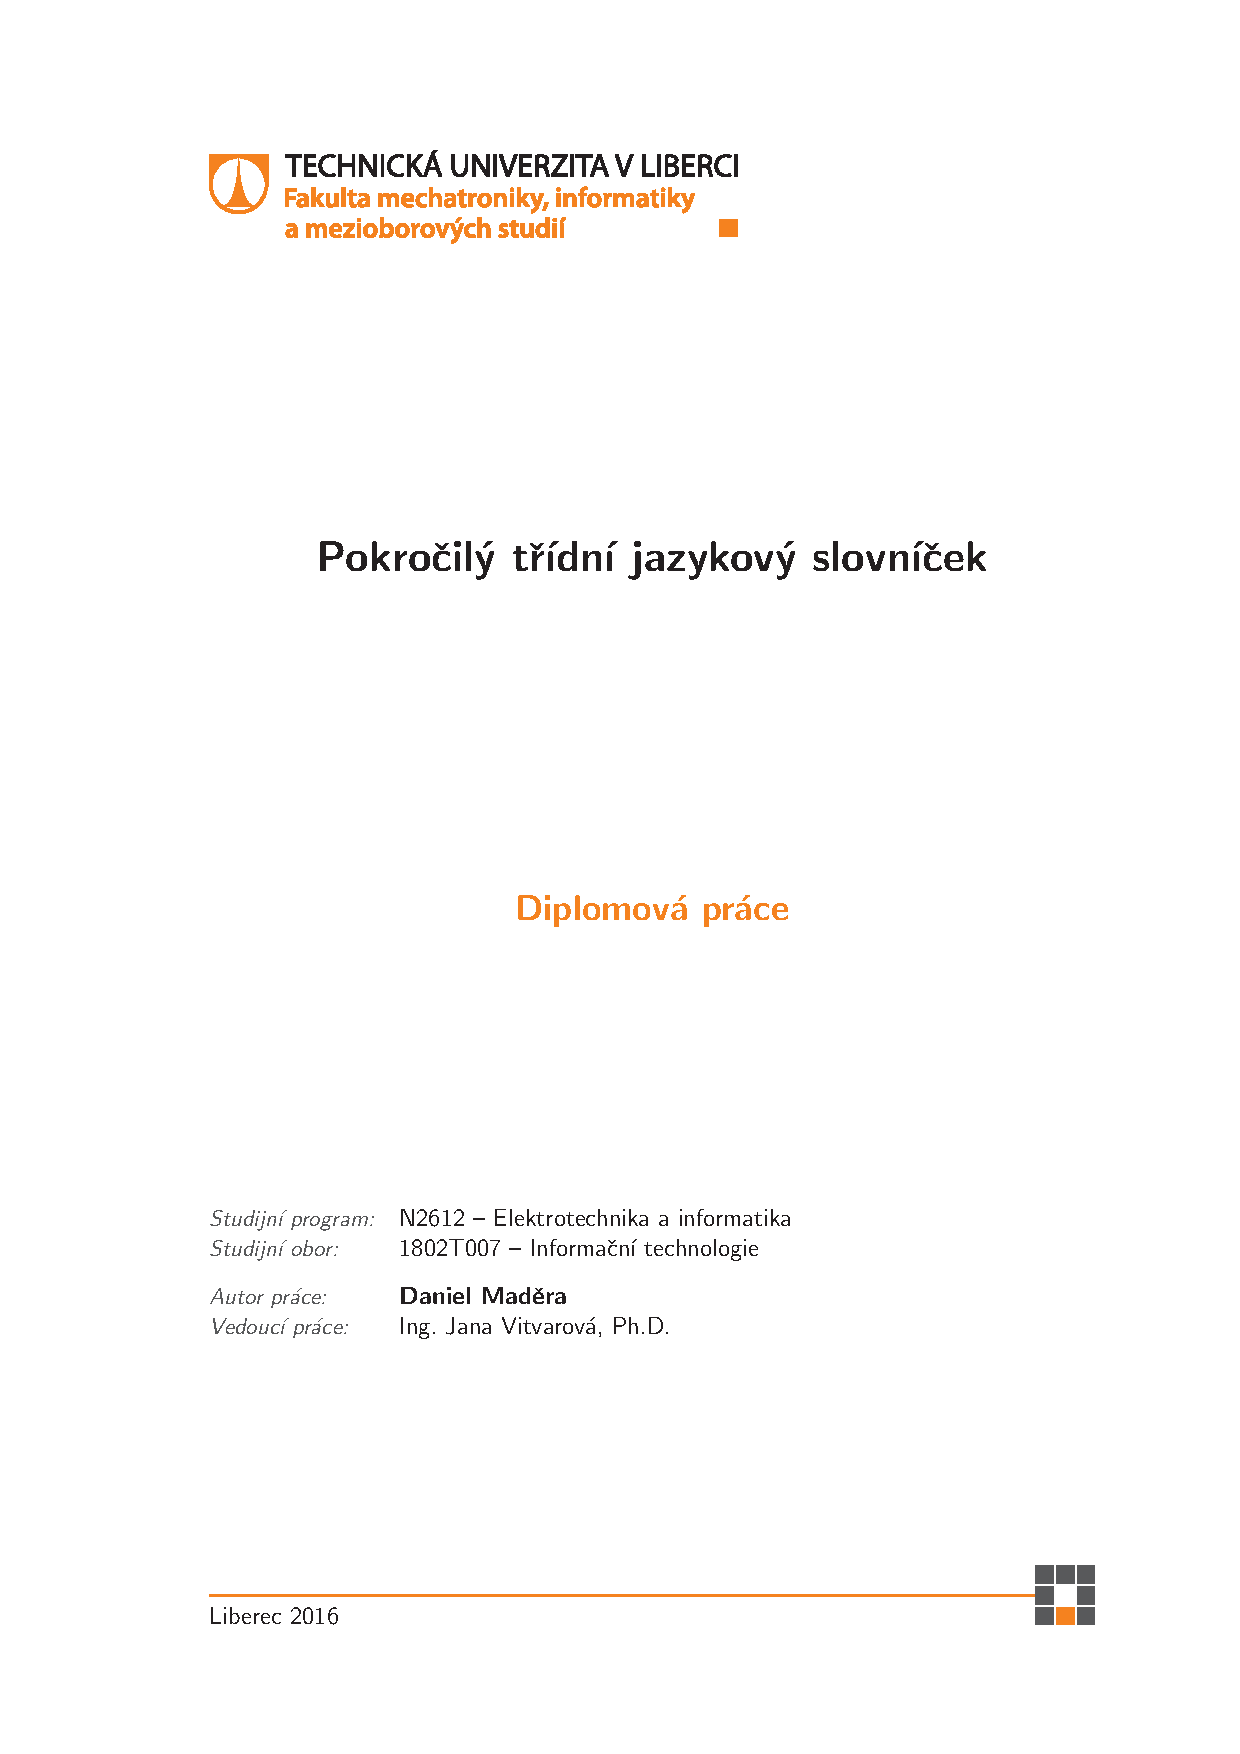
\includepdf[pages={1,2,3}]{dp-titlepage.pdf}
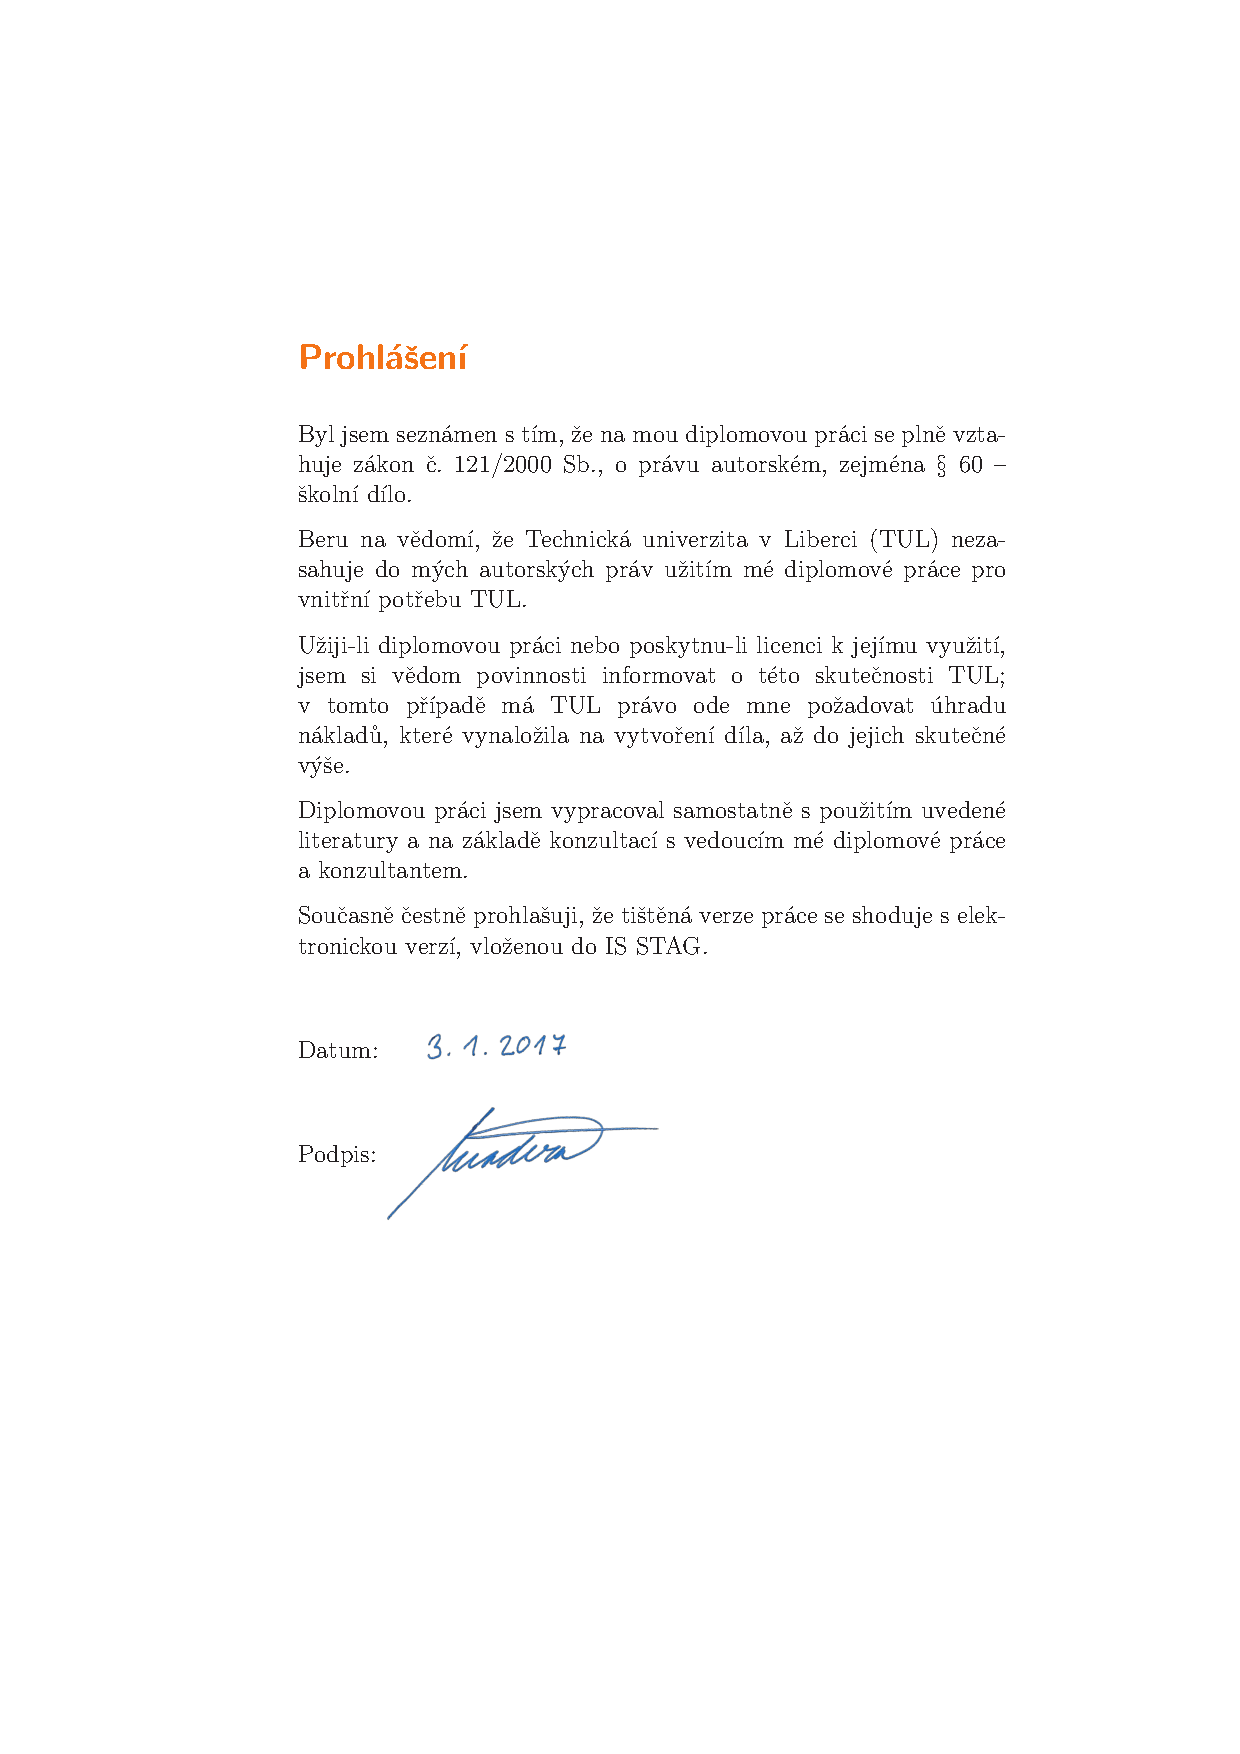
\includepdf{prohlaseni.pdf}
\setcounter{page}{3}

\newpage
\thispagestyle{plain}
\section*{Abstrakt}
% 250 až 500 slov

\section*{Klíčová slova}
% 5 klíčových slov

\thispagestyle{empty}
\newpage

\section*{Abstract}
% 250 až 500 slov

\section*{Keywords}
% 5 klíčových slov

\thispagestyle{empty}

\newpage
\setcounter{tocdepth}{2}
\tableofcontents

\newpage
\listoffigures
\listoftables
\lstlistoflistings

\newpage
\printglossary[type=\acronymtype,title=Seznam zkratek]
%\printglossary[style=altlist,title=Slovník]
\cleardoublepage


\section{Úvod}
    % proč se zaobývat tímto tématem
    % neopakovat abstrakt, lehce nastínit zadání, jaká je motivace
    % popsat, jak je práce strukturovaná - rozcestník


\newpage
\section{Analýza}
    Výuka cizích jazyků je pro aktuální společnost jedna z nejzásadnějších otázek, ať se jedná o pracovní příležitosti v zahraničí, tak sociální problematika světa. Žáci a studenti se často účastní různých kroužků nebo později studenti využívají Erasmus programů, kde vyhledávají právě zlepšení komunikace v cizím jazyce. 

    \subsection{Hlavní cíle}
        % jak si aplikaci představuji
        % zlepšení přípravy na hodiny cizího jazyka
        % shrnout v odstavci požadavky na aplikaci
        
        Hlavním cílem aplikace je připravit žáky na hodinu cizího jazyka a zároveň přirozeně rozvíjet slovní zásobu, tak aby studenti neztratili motivaci a chuť k poznávání nových výrazů. Dále také umožnit žákům se protestovat a ověřit, zda naučenou sadu slov ovládají. Aplikace by se měla adaptovat na zdatnost a úroveň každého ze žáků. Vyučujícím by aplikace měla usnadnit správu a import slovíček, které třída má umět v rámci dané učebnice a následně předkládat žákům vhodnou slovní zásobu například pro následující lekci.

        \subsubsection{Personalizace}
            % personalizace podle potřeby konkrétní třídy - konrétní učebnice
            % personalizace podle potřeby jednotlivých žáků - generování na základě předcházejících výsledků
            Důležitým cílem aplikace by měla být personalizace podle potřeby jednotlivých žáků a celých tříd. Personalizace na úrovni žáka znamená přistupovat individuálně na základě jeho úrovně znalostí a dovedností. V případě konkrétní třídy jde o individuální přístup a to zejména v sadě slov, které je třeba v přípravě procvičovat. 

        \subsubsection{Motivace}
            Důležitou součástí vzdělávání obecně je motivace. Tedy přimět žáky, aby z vlastní iniciativy chtěli rozvíjet své vědomosti. Problém ale je, že se děti přirozeně neučí z vlastní iniciativy, ale aby uspokojili okolí. Motivace se rozdělují do skupin - vnitřní a vnější nebo pozitivní a negativní \cite{bib:motivace}. V analýze bude zaměřeno pouze na motivační prostředky, které lze zařadit do aplikace pro procvičování slovíček.

            Motivace založená na základě vlastních úspěchů je důležitá pro utvrzení sebevědomí žáků. Ocenění v případě zvládnutí sady slov nebo gramatického bloku lze v případě aplikace implementovat například hláškami s projevem pochvaly nebo jiným upozorněním na dosažený výsledek. Zajímavým prvkem v aplikaci by mohlo být i herní prostředí. Žáci si rádi hrají a již J. A. Komenský poukázal na důležitost her ve vzdělávacím procesu.

            % motivace dětí k učení slov (vrámci třídy)
            % motivace - přispění k úspěchu třídy
            % motivace - vlastní úspěchy

            Jedním z dalších stěžejních faktorů motivace je kolektiv. Právě díky kolektivu, ve kterým funguje přirozená rivalita, jsou schopni žáci dosáhnout mnohem vyšších výsledků než kdyby se vzdělávali odděleně a samostatně. Rivalita a soutěživost může projevovat i velmi negativním způsobem. Místo kamarádských vztahů mezi dětmi mohou vznikat nepřátelské, kde může docházet i k posměchu těch, kteří nemusí mít pro výuku až takové nadání. Zajímavější motivací tedy pro kolektiv je například vidina společně dosažených výsledků. V případě učení slovíček by to byl počet slovíček naučených za rok jako celá třída. Dochází zde k utužování kolektivu a děti by mohlo těšit to, že nějakým způsobem přispívají k úspěchům celé třídy.

        \subsubsection{Využití IT pro výuku}
            Posledních několik let se společnost ubírá trendem informačních technologií. Každý ze žáků má už od útlého věku přístup k počítači nebo k chytrému telefonu. Orientace a schopnost tyto zařízení používat není pro ně žádný problém. Přirozeně se tedy tyto zařízení postupně stávají součástí každodenní přípravy žáka na následující školní den. V některých případech tyto zařízení plně nahrazují klasické učebnice a jsou přímo začleněny do výuky. Použití informačních technologií má za následek i zlepšení motivace při výuce. Obecně je známo, že žáci raději studují slovíčka interaktivní formou hádanek, křížovek nebo her, než nekonečných seznamů slov.

            Důležitost cizích jazyků se projevuje na míře používání například chytrých tabulí nebo tabletů při výuce. Tyto zařízení umožňují interaktivní výuku, kde lze využít nejen textových, ale také obrázkových a zvukových prostředků pro lepší zasazení nově nabytých vědomostí do kontextu. 

            % výuka cizích jazyků - smartboards            
            % vysoká motivace dětí pracovat s PC

    \subsection{Existující řešení}
        Na trhu lze nalézt nepřeberné množství aplikací pro výuku cizích jazyků. Řada z nich jsou téměř komplexní systémy, které provází studenta od základních frází a slovíček až po gramatické standardy cizího jazyka. Analýza existujících řešení byla zaměřena na aplikace, které se zabývají především testováním slovíček a frází.

        Do analýzy existujících řešení byly zahrnuty tři desktopové, jedna webová a jedna mobilní aplikace.

        \subsubsection{TS Angličtina}
            Z analyzovaných řešení se jevila desktopová aplikace TS Angličtina od firmy Terasoft ta nejlépe funkčně propracovaná. Tato firma se zabývám širokou škálou výukových nástrojů se zaměřením na základní školy. V případě cizích jazyků se zabývají výukou anglického a německého jazyka. Hlavní předností aplikace je podpora nejvíce používaných učebnic cizího jazyka. Aplikace umožňuje testování různými způsoby - psaný překlad slova, porozumění mluvenému slovu, vybírání správných významů nebo doplňování vynechaných slov \cite{bib:terasoft}. Analýza byla tvořena pouze z informací vydavatele. Bohužel firma Terasoft neposkytuje DEMO nebo TRIAL verzi aplikace, která by hlubší analýzu umožňovala.

        \subsubsection{Langsoft Teacher}
            Dalším analyzovaným řešením byla aplikace Langsoft Teacher, která je dostupná v podání desktopové aplikace, ale také i mobilní aplikace pro platformy iOS a Android. Aplikace je velmi komplexní, obsahuje různé moduly pro testování například v obrazové formě pro předškolní děti. Zajímavá vlastnost, kterou aplikace disponuje, je pamatování problematických slov a nabízení těchto slov častěji než těch bezproblémových. Dále program umožňuje automaticky rozšiřovat slovní zásobu, která je v testování zahrnuta \cite{bib:langsoft}.

        \subsubsection{Duolingo}
            Dalším v pořadí byla aplikace Duolingo. Jedná se o mobilní aplikaci pro Android. Zahrnuje učivo cizího jazyka od základních komunikačních frází až po tvorbu gramaticky složitějších vět. V aplikaci je připravena dlouhá řada cizích jazyků - němčina, angličtina, španělština (kastilština), italština a další. Chybí ale více referenčních jazyků. Aktuálně lze využít pouze angličtinu. Aplikace kromě standardních funkcí zahrnuje i rozpoznávání mluvených odpovědí. Zajímavým poznatkem byl systém motivace uživatelů, kde si každý mohl pozvat své přátele, mezi kterými docházelo k sdílení dosažených výsledků. Dalším motivačním základem bylo nutkání udržení plánu pravidelného testování, jelikož v opačném případě docházelo k automatickému zvyšování objemu testovacích dat. Nevýhodou aplikace byla nutnost připojení k internetu. V případě požití mobilních dat, docházelo ke zpoždění zejména při rozpoznání slov.

        \subsubsection{Vocabulary Trainer}
            Vocabulary Trainer je webová aplikace zdarma napsaná v jazyce PHP, která naučí 5000 nejvíce používaných slov daného jazyka. Aplikace umožňuje hodně možného nastavení. K dispozici je i řada jazyků včetně češtiny a to jako referenční i jako učený jazyk. Testování spočívá nejdříve ve čtení slov a následně uživatel vybírá možnosti odpovědi. Aktuálně překládané slovo si lze kdykoliv přehrát v různé rychlosti. Jako motivační základ aplikace využívá jednoduchý bodový systém. Součástí je i kalendář s email upomínkou k dalšímu testování. Program je propracovaný, ale poměrně pomalý a dlouho trvá zejména úvodní načítání dat. Její výrobce LanguageCourse S.L. poskytuje i mobilní aplikaci pro Android k učení anglických slov a frází.

        \subsubsection{Supermemo aplikace}
            Za zmínku ještě stojí aplikace Supermemo. Není to aplikace s připravenými daty k testování slov cizího jazyka, ale slouží čistě jako šablona pro testování jakéhokoliv druhu otázek. Aplikace implementuje algoritmus Supermemo, který je založen na metodě postupného zvyšování intervalu dotazování na dané otázky. Při každé odpovědi program spočítá, kdy by si uživatel měl danou otázku zopakovat tak, aby odpověď byla správná a zároveň se co nejvíce zvyšoval interval mezi aktuální a předchozí odpovědí. Aplikace se adaptuje na schopnosti uživatele, v přiměřeném měřítku buď zvyšuje nebo snižuje interval dalšího připomenutí.

        % možné ještě rozvést aplikaci EasyWords

        % žádná z aplikací neumožňuje personalizované učení 
        % ve škole (z učebnice) se učí jiná slovíčka než v aplikacích
        % po otestování slova nedochází k jeho znovu připomenutí

        Z výše uvedených aplikací až na Supermemo žádná neumožňuje personalizovaný výběr učiva. Tedy nelze vložit vlastní slovíčko nebo si určit sadu slov pro testování. Proto jsou tyto aplikace především cílené pro uživatele, kteří vnímají výuku jazyka jako samostatné vzdělávání sami sebe. Pro studenty, kteří absolvují lekce z cizího jazyka ve škole je tento typ vzdělávání nevyhovující, jelikož se musí učit dvě nezávislé skupiny slov. Sice dochází k rozvinutí slovní zásoby studenta i do jiných okruhů než je jeho učebnice a málokterý student má ještě energii, časovou dotaci a vlastní iniciativu na to, aby se připravoval na školní test ze slovíček a ještě rozvíjel samostatně svoji cizojazyčnou slovní zásobu.

    \subsection{Učení slovíček}
        % problematika malých dětí a učení slov
        % Biemiller and Boote (2006)
        % ročně se dá zvládnout maximálně 400 slov u studentů 2 - 5 třídy
        % docházelo k zvýšení učenlivosti, když studenti si mohli zapsat 
        % slovo vlastní definicí
        Standardní učení slovní zásoby cizího jazyka je založeno na častém opakování slov. Dle výzkumu Biemillera a Boote se lze ročně zvládnout až 400 slov u studentů 3.—6. tříd \cite{bib:beimiller}. Což v případě cizího jazyka poměrně velké číslo, ale problém je, do jaké míry je slovo správně ukotveno v dlouhodobé paměti. Porovnání, kolik je potřeba slov pro ovládnutí anglického jazyka, usnadní následující tabulka \ref{tab:english-vocab-usage}, která zahrnuje procentuální využití nejvíce používaných slov v každém z odvětví \cite{bib:learning-vocab}. 

        \begin{table}[ht!]
            \centering
            \begin{tabular}{|l|c|c|c|}
            \hline
            & \multicolumn{1}{l|}{Konverzace} & \multicolumn{1}{l|}{Noviny} & \multicolumn{1}{l|}{Akademický text} \\ \hline
            1. 1000 slov & 84,3\% & 75,6\% & 73,5\% \\ \hline
            2. 1000 slov & 6\% & 4,7\% & 4,6\% \\ \hline
            Akademické výrazy& 1,9\% & 3,9\% & 8,5\% \\ \hline
            Ostatní & 7,8\% & 15,7\% & 13,3\% \\ \hline
            \end{tabular}
            \caption{Používání slov v britském anglickém jazyce}
            \label{tab:english-vocab-usage}
        \end{table}

        \subsubsection{Zastaralý způsob učení}
            Dle vlastního průzkumu žáci základních škol nevyužívají k učení slovíček nikterak pokročilé technologie. Většinou si udržují vlastní slovníček, do kterého nově nabytá slova. Při učení zakrývají část s cizími slovy a na základě českého ekvivalentu se snaží vybavit překlad slova. Tato metoda neposkytuje prakticky žádnou zpětnou vazbu. Žáci většinou pouze do krátkodobé paměti uloží slova, později při testu rychle zodpoví a následně během pár hodin si na slovo už ani nevzpomenou. Nevýhod a námětů na zlepšení metody má tato metoda celou řadu, ale jedním z klíčových vad je, že žáci si nevytvoří dostatečně souvislostí, aby řádně ukotvilo slovo v paměti.

        \subsubsection{Zvuková interpretace}
            Zejména v učení cizího jazyka je zvuková podoba a interpretace slov velice důležitá. Jelikož každý jazyk může hlásky různě zvukově interpretovat a pro nováčka v cizím jazyku nemusí textová výslovnost plně vyhovovat. Žák dále díky znění slova získá podvědomí o dialektu daného jazyka a zároveň dochází k lepšímu zapamatování slova. Právě díky zvukům dochází k propojení při učení i pravé mozkové hemisféry. A napomáhá tedy k vytvoření pevnější ukotvení v paměti. Dle studie bulharského vědce George Lozanova, který se zabýval studiem mozku a učebních metod, byl zjištěn obrovský přínos zvukových vjemů \cite{bib:suggestology}.

        \subsubsection{Problematika obtížnosti}
            % každý z žáků má indiviální úroveň znalostí cizího jazyka
            % a každý z žádů se jiným tempem učí cizojazyčná slovíčka
            Velkým problémem v učení slov je přizpůsobit obtížnost každému ze žáků individuálně. Jelikož ne všichni mají stejnou úroveň znalostí cizího jazyka a každý potřebuje jiné tempo pro zapamatování sady slov. Jsou žáci s výbornou pamětí, kterým stačí si slova pouze jednou projít a dokáží je používat, ale jsou žáci, kde nestačí je pětkrát zopakovat. Dalším problémem obtížnosti je z pohledu jednotlivých slov. Každé slovo má odlišnou obtížnost, které lze soudit například podle míry používanosti v jazyce, délky slova, zdali obsahuje přehlasování, dvojitá písmena nebo podobnost s referenčním slovem.

        \subsubsection{Učení slov v kontextu}
            % jak je důlžité se slova učit v kontextu - použití ve větě z učebnice
            % drive/vocab-techniques.pdf
            Pro učení slov cizího jazyka je rovněž důležité správné zasazení významu slova do kontextu. Dle průzkumu Biemillera a Bootea z roku 2006 bylo zjištěno, že u žáků od 10—13 let docházelo k nárůstu zapamatovaných slov o 4\%, pokud byla slova předložena v kontextu vět. Důležitým poznatkem z toho průzkumu je, že žáci si nejen déle naučené slovo pamatovali, ale správně ho i interpretovali, když měli za úkol ho svými slovy vysvětlit \cite{bib:beimiller}. Ve stejném průzkumu rovněž docházelo ještě k vyššímu zlepšení v učení, kdy si žáci zapisovali vlastními slovy definici a použití slova. 
        
    \subsection{Testování slovíček}
        % drive/accesing-vocabulary-in-the-language-classroom.pdf
        % důležitost aktivní slovní zásoby pro výuku cizího jazyka

        \subsubsection{Aktivní a pasivní slovní zásoba}
            % co je aktivní a pasivní
            Slovní zásobu, kterou využíváme k tvorbě vět ať už v cizím nebo mateřském jazyce rozdělujeme na dvě skupiny - aktivní a pasivní. Pasivní zásoba je sada slov, která jsou pevně a spolehlivě uložena v naší paměti. Průměrný žák zná cca 50 000 výrazů. Její velikost je ovlivněna věkem, vzděláním a četbou. Slova ze této sady využíváme zejména při písemné formě, ať už se jedná o čtení nebo psaní. Aktivní zásoba je sada slov, ve které lze najít žádané slovo během desítek milisekund. U většiny lidí dosahuje velikosti 4 000 až 8 000 výrazů \cite{bib:lexikologie}. Slovo se díky používání dostává z pasivní do aktivní slovní zásoby. 

        \subsubsection{Metody testování}
            \label{test-methods}
            % pasivní vs aktivní
            % aktivní - vzpomenutí, rozpoznání

            Metod testování slovní zásoby je mnoho. Základním rozdělením je na pasivní a aktivní. V případě pasivního se jedná například o výběr z nabídnutých možností. Jde o případ, kdy student nemusí znát přesnou odpověď a dokáže otázku vyhodnotit správně vylučovací metodou. Při aktivním testování žáci musí odpověď znát, aby otázka byla vyhodnocena správně. Pasivní metoda má pozitivní vliv například na motivaci žáka, který u ní tolik netápe a za pomoci zdravého rozumu může test vyhodnotit správně. Problém ale vzniká při používání získaných a procvičených informací. V případě cizího jazyka lze pasivní slovní zásobu využít pro čtení a náslech, ale pro ovládnutí cizího jazyka je nedostatečná a tudíž nevhodná. 

            Dalším rozdělením pasivního a aktivního testování slovíček je rozpoznávání (\textit{recognition}) a vzpomenutí (\textit{recall}). Rozpoznávání spočívá v předložení cizího slova žákovi a pro správné zodpovězení musí najít český ekvivalent. Vzpomenutí je způsob testování opačným způsobem než rozpoznání. Tedy uživateli je předložen výraz v jeho mateřském jazyce a on musí nalézt správný výraz v cizím. Rozpoznání je z principu jednodušší pro uživatele než vzpomenutí. Lze ho tedy využít rovněž pro zvýšení motivace při procvičování slov. Ale pro ověření, zda je slovo ovládnuté či nikoliv je metoda rozpoznání také nedostatečná.

        \subsection{Typy testů}
            % multiplechoice, matching, completion, translation
            % vyžití her - problém je, že tento způsob většinou není ani efektivní, jelikož si procvičí například v případě doplňování písmen pouze pár slov za poměrně dlouhý čas

            V analýze existujících řešení bylo procvičování a testování slov interpretováno různými způsoby. Obecně by se typ testů dal rozdělit na tři kategorie - textové testy, multimediální a herní testy.

            \subsubsection{Textové testy}
                Textové testy se vyskytovaly například jako výběr z více možností nebo spojováním spolu souvisejících významů, jak už ale bylo uvedeno v kapitole \ref{test-methods}, jedná se o rozvíjení pasivní slovní zásoby. Zajímavějším typem testů je doplňování slov do vět a klasický překlad slova. Tyto typy rozvíjejí žádanou aktivní slovní zásobu. Standardně textové testy byly doplněny zvukovou interpretací cizího slova.

            \subsubsection{Multimediální a herní testy}
                Zajímavým využitím multimédií by mohlo být zahrnutí otestování výslovnosti. Tedy možnost nahrání odpovědi a následně by došlo k rozpoznání. Ale analýza a rozpoznání řeči není nikterak triviální záležitost. Dalším zajímavým řešením byly herní testy. Díky nimž docházelo k zvýšením motivace uživatelů. Problém je, že tento typ procvičování většinou není zas tolik efektivní, jelikož si uživatel procvičí například v případě doplňování písmen křížovky nebo známé hry \textit{Hangman} pouze pár slov za poměrně dlouhý čas.  

    \subsection{Specifikace požadavků}
        % číselný seznam toho, co má aplikace dělat
        Na základě analýzy byla provedena specifikace požadavků, které budou implementovány v aplikaci pro testování slovíček z cizího jazyka.

        \begin{enumerate}
            \item správa učebnic
                \begin{itemize}
                    \item tvořit, editovat a mazat vlastní učebnice
                    \item umožnit publikovat učebnici pro veřejnost
                \end{itemize} 
            \item správa slovíček v učebnici
                \begin{itemize}
                    \item tvořit, editovat a mazat slovíčka
                    \item hromadně slovíčka do učebnice importovat
                    \item částečně automatizovat zvukovou a obrazovou interpretaci slovíčka
                \end{itemize} 
            \item správa modulů a tématických okruhů v učebnici
                \begin{itemize}
                    \item tvořit, editovat a mazat moduly a tématické okruhy učebnice
                    \item přiřazovat slovíčka do daných modulů a okruhů
                \end{itemize}
            \item správa uživatelských skupin (tříd)
                \begin{itemize}
                    \item tvořit, editovat a mazat uživatelské skupiny
                    \item umožnit uživatelům se přihlásit do skupiny
                \end{itemize}
            \item správa testovacích sad
                \begin{itemize}
                    \item tvořit, editovat a mazat testovací sady
                    \item umožnit vybírat slova pro testovací sadu z vlastních i veřejných učebnic
                    \item přiřazovat testovací sady ke skupinám uživatelů
                \end{itemize}
            \item procvičování slovíček
                \begin{itemize}
                    \item vybrat testovací sadu slovíček
                    \item generovat slova na základě úrovně uživatele
                    \item zahrnout obrazovou a zvukovou interpretaci do procvičování
                    \item možnost uložit stav testování a umožnit pozdější navázání
                \end{itemize}
            \item připomínat a procvičovat ovládnutou slovní zásobu 
            \item motivace
                \begin{itemize}
                    \item motivovat v rámci uživatelské skupiny
                    \item motivovat vlastní iniciativu k procvičování
                \end{itemize}
        \end{enumerate}


\newpage
\section{Návrh aplikace}
    % usecase diagram
    % jednotlivé use-case by měly být názvy jednotlivých podkapitol v návrhu aplikace
    Na základě specifikace požadavků byl vytvořen USE-CASE diagram aplikace. Diagram na obrázku \ref{fig:use-case} znázorňuje pouze obecné bloky funkčnosti aplikace. V následujících kapitolách bude každý z jednotlivých USE-CASE bloků popsán detailněji.

        \begin{figure}[ht!]
            \centering
            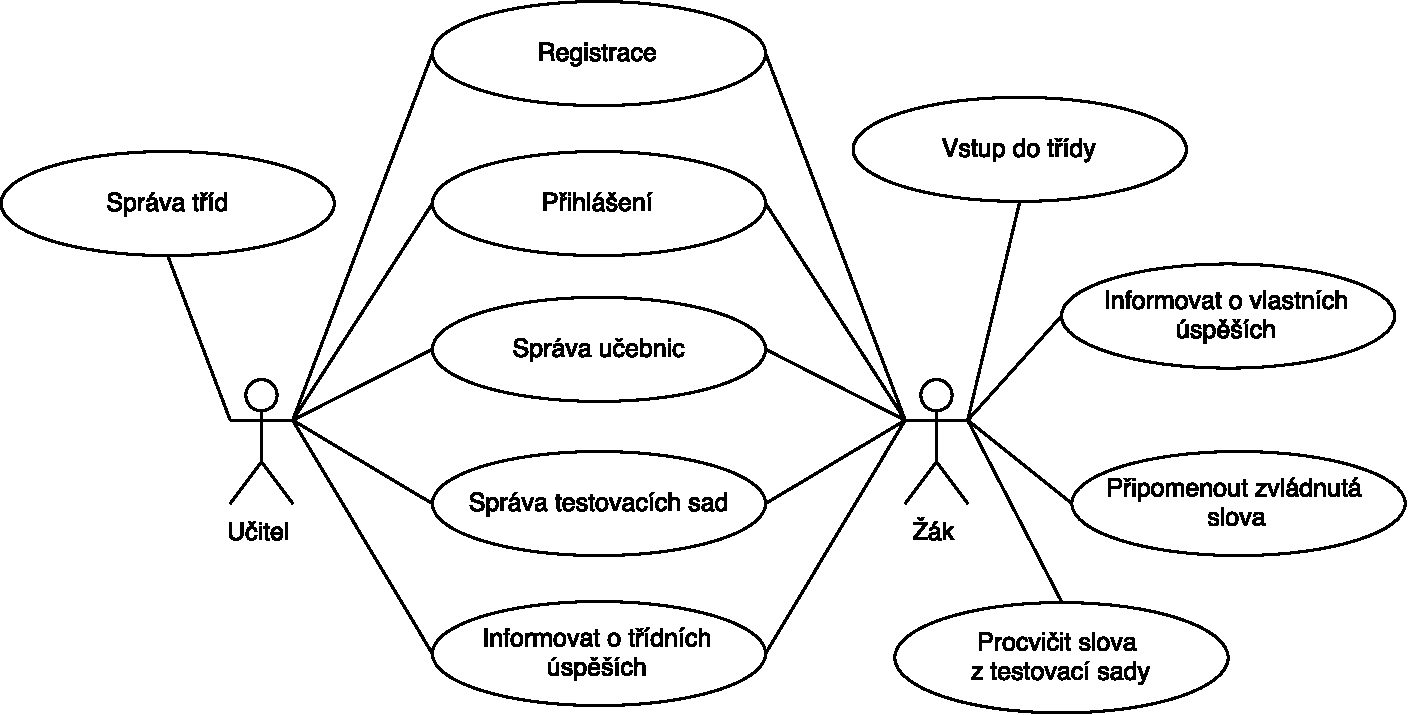
\includegraphics[scale=0.63]{../diagrams/use-case.pdf}
            \caption{USE-CASE diagram aplikace}
            \label{fig:use-case}
        \end{figure}

    \subsection{Uživatelské role}
        % rozvést rozdíl mezi žákem a učitelem - rovnocenné partnerství, každý může být učitel a student
        Do aplikace by měly vstupovat dva typy uživatelů - učitel a žák. Učitel z principu má za úkol spravovat testovací sady, učebnice a třídy. Žáci oproti nim mají za úkol vstupovat do svých tříd, procvičovat slova z testovacích dat, které jsou připravené od učitele a připomínat si zvládnutá slova. 

        Po konzultacích s vedoucím práce a vyučujícím cizího jazyka na základní škole došlo k několika změnám v návrhu právě v oblasti uživatelských rolí a i v principu aplikace. Vznikl požadavek, že aplikace by mohla fungovat spíše jako portál pro vzdělávání a ne jako výukový nástroj pro učitele. V návrhu tudíž vzniklo rovnocenné partnerství mezi učitelem a žákem.

        \subsubsection{Sjednocení uživatelským skupin}
            Podnětem pro sjednocení uživatelských skupin vedlo umožnění žákům procvičovat si slova i v případě, že nejsou součástí žádné třídy. Tak aby mohl kdokoliv se do aplikace přihlásit, vybrat si testovací sadu a vyzkoušet svoje znalosti slovíček. Tato funkce umožňuje žákům volnější přístup k výuce. Nebylo totiž v požadavcích to, aby učitel měl přehled o znalostech žáka - právě naopak. Účelem aplikace je poskytnout žákům možnost se samostatně vzdělávat a procvičovat slovní zásobu a ne vyučujícím poskytnout nástroj pro otestování, zda žák disponuje požadovanými znalostmi. 

    \subsection{Správa učebnic}
        % sdílení učebnic (otevřený systém)
        % přijít do aplikace a jen tak si protestovat slova z učebnice
        % nemusí být člověk součástí žádné skupiny
        Z důvodu personalizace slovíček bylo nutné v návrhu aplikace zařadit učebnice, díky nimž si žáci budou procvičovat pouze slovíčka, která jsou pro ně aktuální ve výuce cizího jazyka. Učebnice obsahují moduly a v modulech se nacházejí jednotlivá slova. Při tvorbě učebnice bude zvolen cizí jazyk, pro který je učebnice připravená. V rámci jedné učebnice jsou slova unikátní. Tzn. do konkrétní učebnice nemohou patřit dvě stejná slova. Majitel učebnice je může editovat, vytvářet, skrýt pro veřejnost a mazat i v případě, že je využívána některým z ostatních uživatelů. 

        V aplikace se může vyskytovat i více stejných učebnic. Například dva různí vyučující vedou své hodiny cizího jazyka dle stejné učebnice, ale každý si chce přizpůsobit sadu slov po svém. Proto se v aplikaci musí učebnice identifikovat majitelem a názvem učebnice.

        \subsubsection{Sdílení učebnic}
            Jelikož aplikace slouží jako portál pro vzdělávání, ve výchozím stavu jsou učebnice a slovíčka v nich veřejně přístupné jakémukoliv uživateli. Příchozí uživatel si tedy bude moci buď vytvořit vlastní učebnici se svými slovy, které si chce procvičit nebo může vyhledat už z vytvořených učebnic. Díky sdílení nový uživatel může prakticky okamžitě po přihlášení začít procvičovat slova a nemusí složitě žádná slova importovat. Tento přístup je cílený právě především pro žáky, kteří si chtějí samostatně procvičovat slova a nepatřit do žádné konkrétní třídy.


    \subsection{Správa slovíček}
        % výhody více forem - lepší zapamatovatelnost
        % vytvoření hlubších asociací

        Jednotlivá slovíčka se budou ukládat do daným modulů učebnice. Slovíčko se bude charakterizovat - překladem v cizím jazyce, významem v mateřském jazyce, definice slova v cizím i mateřském jazyce a použití ve větách z učebnice. Dalšími atributy, kterými slovíčko bude disponovat, jsou obtížnost a slovní druh. Slovíčko bude možné doplnit o multimediální interpretaci a to v podobě zvuku a obrázku.

        %% Možné rozšíření - přidat možnost více významů slova
        \subsubsection{Textová forma}
            % importováním sady slov (bez automatizace překladů)
            % editace definic a použití ve větách
            Textová forma slovíčka spočívá v překladu slova a jeho významu v mateřském jazyce. Pro zjištění významu slova se může využít již hotové aplikace. Například Google Translate poskytuje aplikační rozhraní pro překlady slov i celých vět. Výhodou by bylo usnadnění zadávání a import slovíček do aplikace. Jelikož se aplikace bude zabývat aktivním rozpoznání a vzpomínání, je vhodné neautomatizovat významy slov. Učebnice nebo učitelé se mohou s Google Translate lišit v definování významů slov. Dalším problémem je cena využívání překladů z Google Translete, která je účtovaná měsíčně a to \$20 za 1 milion znaků \cite{bib:google-api}.

        \subsubsection{Zvuková forma}
            % z Google API importovat zvukové nahrávky
            % shrnout omezení, problematiku
            % 60 minut měsíčně je zdarma
            Do aplikace by měla být implementována i zvuková interpretace slovíčka v cizím jazyce. Zvukové nahrávky mohou být zařazeny do aplikace dvěma způsoby - manuálně vlastními nahrávkami nebo využít Google Text to Speech API, které poskytuje zdarma, pokus se měsíční využití zvukových nahrávek obsáhne do 60 minut\cite{bib:google-api}. V případě jedno nebo dvouslovných spojení, které zaberou přibližně 4—8 vteřin, je dostačující pro cca 600 slovíček za měsíc. Aplikace bude záznam lokálně ukládat, aby bylo se co nejvíce omezilo využívání API. Zvuková nahrávka bude získána při importu slovíček do učebnice. Zadávající uživatel si bude moci zvolit, k jakému slovu chce zvukovou interpretaci.

        \subsubsection{Obrazová forma}
            % vyhledání z Google Images API na základě cizojazyčného slova
            % autor učebnice vybírá dané slovo z importovaných
            % omezení dotazů - neprovádí se plně automatiky
            Obrazová interpretace slovíčka bude rovněž získaná z Google Custom Search API. Toto aplikační rozhraní není omezené a lze v parametrech omezit vyhledávání pouze na obrázky. Při importu si uživatel zvolí pro jaká slovíčka chce obrazovou formu. Automatizace v tomto případě není vhodná, jelikož ne všechny slovíčka lze interpretovat jako obrázek. Uživatel si také bude moci zvolit obrázek z několika možností. Po vybrání obrázku bude vytvořena komprimovaná kopie souboru a uloží se rovněž zdroj, odkud je obrázek získán. Tato forma bude v aplikaci sloužit pouze jako nápověda pro žáky, díky níž si mohou ke slovíčku vytvořit hlubší asociaci. 

            % využití možnost hledání dle "Lze volně užívat nebo sdílet". Vytvoření kopie, 
            Díky Google Custom Search API lze vyhledávání parametrizovat. Výrazem pro vyhledávání bude referenční slovo v cizím jazyce, jelikož cílový jazyk bude nejspíš anglický, německý nebo španělský a všechny tyto jazyky jsou více rozšířené než ten český. Dalším parametrem vyhledávání je omezení pouze na obrázky s licencí a \uv{Volně užívat nebo sdílet}, která umožňuje obrázek zkopírovat a nekomerčně publikovat s uvedením zdroje. Bohužel společnost Google Inc. nezaručuje pod jakou licencí obrázek aktuálně se na stránkách prezentuje. Proto bude uživatel při výběru obrázku vyzván, aby zkontroloval licenci použití.

    \subsection{Obtížnost slovíček}
        % vygenerovaná obtížnost na základě délky slova, podobnosti s českým jazykem, přizpůsobena vyučujícím
        Při zadávání slova do učebnice bude automaticky vyhodnocena jeho obtížnost, která je rozdělena do čtyř kategorií - snadné, střední, těžké a nemožné. Vyhodnocení obtížnosti je založeno na kombinaci několika parametrů slova - jeho délky, podobnosti s českým ekvivalentem a další atributy jako počet přehlasovaných písmen nebo počet výskytů dvojitých písem. V případě nevhodně vygenerované obtížnosti slova, uživatel ji bude moci opravit dle vlastního uvážení. Délka slova je prahově rozdělena do kategorií obtížnosti, následně bude vyhodnocena podobnost s významem pomocí Levensteinovy vzdálenosti popsané v podkapitole \ref{levenstein}. Poté následuje vyhodnocení přehlasování a dvojitých hlásek, které ale ovlivňují obtížnost už minimálně.

        \subsubsection{Výběr algoritmu}       
            Levenshteinova vzdálenost je velmi podobná známe Hammingově vzdálenosti s tím rozdílem, že Hammingova vzdálenost uvádí počet pozic se stejným symbolem v obou řetězcích. Kdežto Levenshteinova uvádí počet jednoznakových editací. Pro určení míry podobnosti mezi slovem v cizím jazyce a jeho překladem je vhodnější Levenshteinova vzdálenost, jelikož akceptuje řetězce s různou délkou a v případě, že písmeno chybí, je to vyhodnoceno pouze jako odstraněné písmeno a algoritmus pokračuje dál. V případě Hammingovy vzdálenosti, vynechané písmeno naruší porovnávání zbytku řetězce.

        \subsubsection{Levenshteinova vzdálenost}
            \label{levenstein}
            Levenshteinova vzdálenost v informatice je míra rozdílu mezi dvěma řetězci. Pro výpočet vzdálenosti se využívá matice s rozměry velikostí délek řetězců. V podstatě vzdálenost je minimální počet jednoznakových úprav ve slově, aby vzniklo slovo referenční. Za jednoznakovou úpravu se považuje smazání, záměna nebo vložení písmene na dané místo.

            Vzorec \ref{levenshtein} je matematický zápis Levenshteinovy vzdálenosti, kde $a$ a $b$ jsou řetězce $a(i)$ a $b(j)$ jsou indexované znaky v řetězcích. Výsledná vzdálenost je rovna hodnotě v matici $dist_{a,b}$ na pozici $dist_{a,b}(|a|,|b|)$, kde $|a|$ a $|b|$ jsou délky řetězců \cite{bib:levenshtein}.

            \begin{ceqn}
            \begin{align}
                \label{levenshtein}
                dist_{a,b}(i,j) = 
                \begin{cases} 
                    max(i,j) & min(i,j) = 0\\min
                        \begin{cases}
                            dist_{a,b}(i-1,j)+1\\dist_{a,b}(i,j-1)+1\\dist_{a,b}(i-1,j-1)+
                            \begin{cases}
                                0 & a(i) = b(j)\\1 & a(i) \neq b(j)
                            \end{cases} 
                        \end{cases} & min(i,j) \neq 0 
                \end{cases}
            \end{align}
            \end{ceqn}

            V případě, že se pohybujeme v matici v prvním sloupci a prvním řádku přiřazujeme hodnoty 1 až délka řetězce $a$ do sloupce a 1 až délka řetězce $b$ do řádku. Tedy první sloupec a první řádek v matici slouží jako referenční inicializace. V generování matice se následně pokračuje a porovnávají se jednotlivé znaky. První položka v minimu je případ, kdy písmeno bylo odstraněno z $a$. Druhá položka je případ, kdy došlo k vložení znaku do a na základě znaku v $b$ řetězci. A poslední položka je případ porovnání znaků. V okamžiku, kdy znaky se rovnají, hodnota vzdálenosti na diagonále zůstává, v opačném případě se přičítá jednička.

            Výpočet Levenshteinovy vzdálenosti dvou slov znázorňuje matice \ref{leven-matice}, kde dochází k porovnání českého slova \textit{cyklus} a anglického výrazu \textit{cycle}. Tučně je znázorněna cesta výpočtu. Prováděné jednoznakové operace jsou žádná, žádná, žádná, záměna, záměna a vložení.

            \begin{ceqn}
            \begin{align}
                \label{leven-matice}
                \begin{matrix}
                    &  & c & y & c & l & e \\
                    & \textbf{0} & 1 & 2  & 3 & 4  & 5 \\
                    c & 1 & \textbf{0} & 1 & 2 & 3 & 4 \\
                    y & 2 & 1 & \textbf{0} & 1 & 2 & 3 \\
                    k & 3 & 2 & 1 & \textbf{1} & 2 & 3 \\
                    l & 4 & 3 & 2 & 2 & \textbf{1} & 2 \\
                    u & 5 & 4 & 3 & 3 & 2 & \textbf{2} \\
                    s & 2 & 5 & 4 & 4 & 3 & \textbf{3} \\ 
                \end{matrix}
            \end{align}
            \end{ceqn}

        \subsubsection{Určení obtížnosti}
            % shrnutí o váženém průměru obtížnosti, jaké a v jaké váze faktory jako Levenshtein, přehlasování a dvojitá písmena tvoří určení obtížnosti slova

    \subsection{Generování slov pro testování}
        % generování slov na základě motivace, obtížnosti 
        % základem je slova, která jsou problematická pro žáka generovat častěji než slova, 
        % která zvládá s přehledem
        % účel generování slov má procvičit slova tak, aby byly správně ukotveny v dlouhodobé paměti a ne pouze v té krátkodobé
        Způsob generování slov je důležité pro správné ukotvení slova v dlouhodobé a ne krátkodobé paměti. Při testování bude docházet i k několika násobnému opakování slova, což popisuje podkapitola \ref{repeating}. Základem generování je častěji a vícekrát předkládat slova, která jsou pro žáka problematická a slova, která jsou zvládnuta žákem s přehledem, budou méně častěji testována. Pro generování byla zvolena metoda rozloženého opakování (\textit{spaced repetition}) popsaná v následujících podkapitolách.

        \subsubsection{Rozložené opakování} % Spaced repetition
            % obecně o metodě 
            Až na výjmečné paměti je obecně známo, že pokud chceme informaci v paměti uchovat dlouhodobě, je nutné opakovaně připomínat. Pokud informace není vyžívána s největší pravděpodobností dojde ke ztráte této informace. V případě, že uživatel s touto informací pracuje častěji, výrazně navyšuje šance pro její zapamatování. Metoda rozloženého opakování je učební technika založená na opakovaném připomínání informace s navyšujícím itervalem. Na začátku učebního procesu, jsou intervaly krátké například na hodinu, 4 hodiny nebo celý den. S postupem se tyto intervaly mohou zvyšují až na týdny a měsíce. Ideální systém rozploženého opakování nabídne zopakování informace těsně před tím, než dojde k jejímu zapomenutí.

            

        \subsubsection{Leitnerův algoritmus}
            % shrnout leitnerův algoritmus
            % The Leitner System can be viewed as a physical box in which you store your flashcards. The box has several compartments labeled e.g. 1 to 5 (you could choose more compartments as well). You then put each of your flashcards into appropriate compartments in this box. If your flashcard is still new you will want to put it in the first compartment, where you repeat the flashcards every day. Flashcards, which you know well will be put into the second compartment. Flashcards in the second compartment have to be reviewed every second day. Flashcards, which you know well there will be moved to the third compartment and so on. Each compartment has a different repetition interval. And flashcards, which you know well, get promoted to the next compartment.
            % In case that you could not answer a flashcard correctly you move it back to the first compartment where the cycle starts again.

        \subsubsection{Opakování slov v testování}
            \label{repeating}

        \subsubsection{Adaptivní a globální obtížnost}


    \subsection{Procvičování slovíček}

        \subsubsection{Metody testování}
            % aktivní rozpoznání a aktivní vzpomenutí
            % algoritmus na záměnu vzpomenutí a rozpoznání (možná obrázek)
    
        \subsubsection{Nápovědy}
            % definice se zobrazuje ihned, kontext slova ve větě z učebnice, první písmeno
            % možnost vyplnění definice slova - (automaticky předvyplnit - volně dostupné definice)

        \subsubsection{Kontrola podvádění}
            % problém, není možné kontrolovat, zda si uživatelé nevyhledávají
            % slova ve slovnících a potom nedoplňují do aplikace
            % měření času odpovědi - v závisloti na délce odpovědi

            % učitel nevidí statistiky dětí, pouze celé třídy
            % aplikace nemá sloužit na zkoušení dětí učitelem
            % testing to learn, not testing to assess        

    \subsection{Vyhodnocování odpovědí}
        % určení vzdálenosti slov - více úrovní odpovědí
        % shrnout levenstein algoritmus

    \subsection{Připomínání slov}
        % shrnout supermemo aplogritmus

    \subsection{Motivace}
        % počty zvládnutých slov studenta
        % třídních zvládnutých slov
        % cinknutí při zvládnutém slově

    \subsection{Model databáze}


    \subsection{Architektura aplikace}
        % architektura celé aplikace
        % 2 části, ve skratce popsat, která je za co zodpovědná


\newpage
\section{Klientská aplikace}

    \subsection{Návrh aplikace}

        \subsubsection{Single-page}
            % definice
            % výhody

        \subsubsection{Model aplikace}
            % url diagram
            % mock api

        \subsubsection{Editovatelné seznamy}
            % editace dat v podobě autosave editovatelných seznamů

        \subsubsection{Design}
            % wireframes
            % responzivnost      

        \subsubsection{Implementace algoritmů}

        \subsubsection{Adaptovaná Levenshteinova vzdálenost}
            % Levenstein a Leitner jsou implementovány na klientské straně

        \subsubsection{Google API}
            % api console key
            % images

    \subsection{Vývojové prostředí}
        \subsubsection{Webpack}
            % css injections, production vlastní css soubor
            % - rychlejší načítání (solo js solo css)

        \subsubsection{Babel}
        \subsubsection{JSX}


    \subsection{Knihovna React}
        
        \subsubsection{Abstraktní DOM}
        \subsubsection{Mobx}
            % knihovna React se stává frameworkem
        \subsubsection{Imutabilita}
        \subsubsection{Směrování}
        \subsubsection{Komponenty}


    \subsection{Implementace technologií}
        % layout komponenta
        % využití Mobx - MVC (stores, components)

        \subsubsection{Adresářová struktura}
        

    \subsection{Testování}
        % Karma, NPM spouštění
        % využití MOBX data injections v daném stavu aplikace


\newpage
\section{Serverová aplikace}
    
    \subsection{Technologie}
        \subsubsection{Webová aplikace}
            % výhody webových aplikací

        \subsubsection{Architektura}
            % architektura klient + server
            % možnost více klientů (mobilní aplikace apod.)

        \subsubsection{HTTP a REST API}

        \subsubsection{WSGI}

        \subsubsection{Implementace algoritmů}
            % Supermemo implementace na serveru
            % CRON připomínací emaily pouze v případě, že stihneš dodělat do APP

    \subsection{Django a REST framework}
        
        \subsubsection{Autorizace}

        \subsubsection{Autentizace}

        \subsubsection{Optimalizace API}

    \subsection{Zabezpečení}

        \subsubsection{HTTP/2}

        \subsubsection{OAuth2}

        \subsubsection{JWT}

        \subsubsection{CORS}

    \subsection{PostgreSQL}

    \subsection{Testování}
        % APITestCase Django REST


\newpage
\section{Závěr}
    %% Možné rozšíření - přidat možnost více významů slova

\newpage
\begin{thebibliography}{99}
    
    \addcontentsline{toc}{section}{\refname}

    \bibitem{bib:terasoft}
        Terasoft, a.s. \textit{Terasoft - Výukové programy} [online] 2002-10-07. [cit. 2016-12-15]. Dostupné z: \url{http://www.terasoft.cz/czpages/cd_aj15.htm}
    
    \bibitem{bib:langsoft}
        LangSoft s.r.o. \textit{Language Teacher} [online]. [cit. 2016-12-07]. Dostupné z: \url{http://www.langsoft.cz/teacher.htm}

    \bibitem{bib:motivace}
        KREJČOVÁ, Lenka. \textit{Psychologické aspekty vzdělávání dospívajících}. 1. vyd. Praha: Grada Publishing, 2011 [cit 2016-12-18]. ISBN 978-80-247-3474-3.

    \bibitem{bib:beimiller}
        BIEMILLER, Andrew, BOOTE, Catherine. \textit{An effective method for building meaning vocabulary in primary grades}. Vol 98(1), Journal of Educational Psychology, 2006 [cit 2016-12-18].

    \bibitem{bib:suggestology}
        LOZANOV, Georgi. \textit{Suggestology and Outlines of Suggestopedy}. 1. vyd. Gordon and Breach, 1978 [cit 2016-12-18]. ISBN 0-203-39282-5.

    \bibitem{bib:learning-vocab}
        I. S. P. Nation \textit{Learning Vocabulary in Another Language}. Cambridge University Press, 2001 [cit 2016-12-18]. ISBN 0-521-800927.

    \bibitem{bib:lexikologie}
        SVOBODOVÁ Jana, SVOBODOVÁ Diana, KULDANOVÁ Pavlína, GEJGUŠOVÁ Ivana, ROSOVÁ Milena, NOVÁK Radomil. \textit{Lexikologie} [online] 2003. [cit. 2016-12-19]. Dostupné z: \url{http://www.osu.cz/fpd/kcd/dokumenty/cestinapositi/lexikologie.htm}

    \bibitem{bib:levenshtein}
         Wikimedia Foundation, Inc. \textit{Levenshtein distance} [online] 2016-12-20. [cit. 2016-12-21]. Dostupné z: \url{https://en.wikipedia.org/wiki/Levenshtein_distance}
        
    \bibitem{bib:google-api}
        Google Inc. \textit{Google Cloud Platform} [online]. [cit 2016-12-21]. Dostupné z: \url{https://cloud.google.com/}
 
\end{thebibliography}
\end{document}
